\documentclass[ignorenonframetext,]{beamer}
\usetheme{default}
\usecolortheme{dove}
\setbeamertemplate{caption}[numbered]
\setbeamertemplate{caption label separator}{:}
\setbeamercolor{caption name}{fg=normal text.fg}
\usepackage{amssymb,amsmath}
\usepackage{ifxetex,ifluatex}
\usepackage{fixltx2e} % provides \textsubscript
\usepackage{lmodern}
\usepackage{tikz}
\ifxetex
  \usepackage{fontspec,xltxtra,xunicode}
  \defaultfontfeatures{Mapping=tex-text,Scale=MatchLowercase}
  \newcommand{\euro}{€}
\else
  \ifluatex
    \usepackage{fontspec}
    \defaultfontfeatures{Mapping=tex-text,Scale=MatchLowercase}
    \newcommand{\euro}{€}
  \else
    \usepackage[T1]{fontenc}
    \usepackage[utf8]{inputenc}
      \fi
\fi
% use upquote if available, for straight quotes in verbatim environments
\IfFileExists{upquote.sty}{\usepackage{upquote}}{}
% use microtype if available
\IfFileExists{microtype.sty}{\usepackage{microtype}}{}

% Comment these out if you don't want a slide with just the
% part/section/subsection/subsubsection title:
\AtBeginPart{
  \let\insertpartnumber\relax
  \let\partname\relax
  \frame{\partpage}
}
\AtBeginSection{
  \let\insertsectionnumber\relax
  \let\sectionname\relax
  \frame{\sectionpage}
}
\AtBeginSubsection{
  \let\insertsubsectionnumber\relax
  \let\subsectionname\relax
  \frame{\subsectionpage}
}

\setlength{\parindent}{0pt}
\setlength{\parskip}{6pt plus 2pt minus 1pt}
\setlength{\emergencystretch}{3em}  % prevent overfull lines
\setcounter{secnumdepth}{0}

\title{Stochasticity and Evolution in Food Webs}
\author{\href{http://gvdr.github.io}{Giulio Dalla Riva}\\ University of
Canterbury, NZ}
\date{Granada Seminar June 16, 2015}

\usebackgroundtemplate{%
\tikz\node[opacity=0.2] {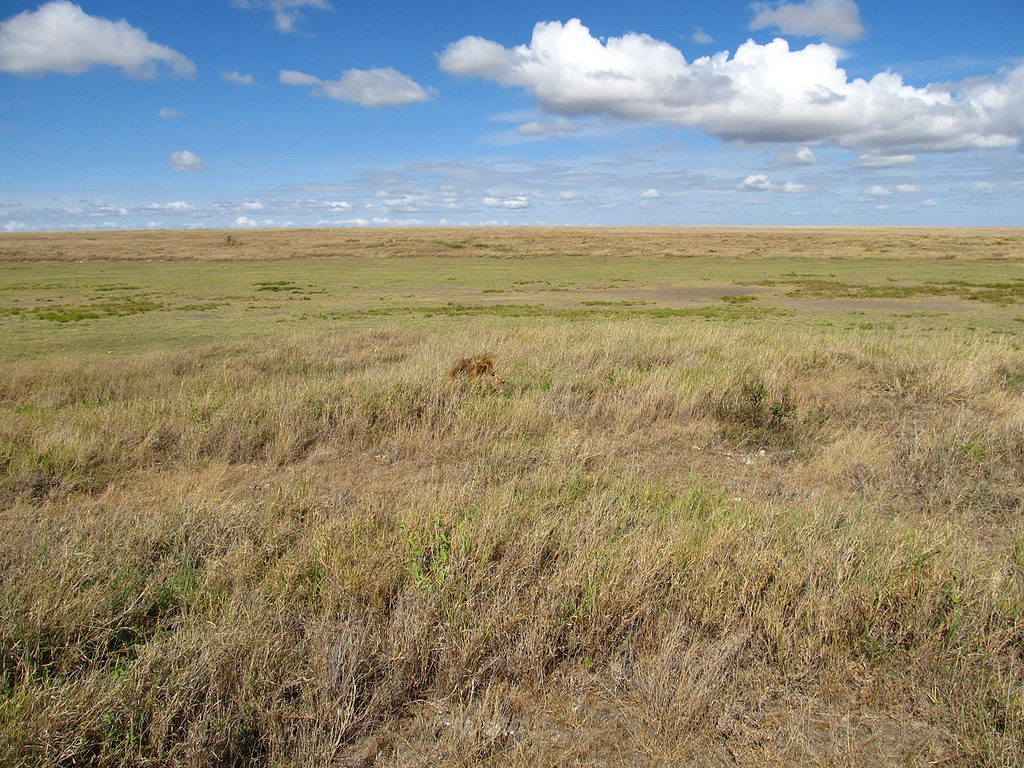
\includegraphics[height=\paperheight,width=\paperwidth]{images/Serengeti_background.jpg}};}

\begin{document}
\frame{\titlepage}

\begin{frame}{species ARE related}

\centering
\begin{tabular}{|c|c|}\hline
Evolution & Ecology \\\hline\hline
Phylogeny & Food Web \\
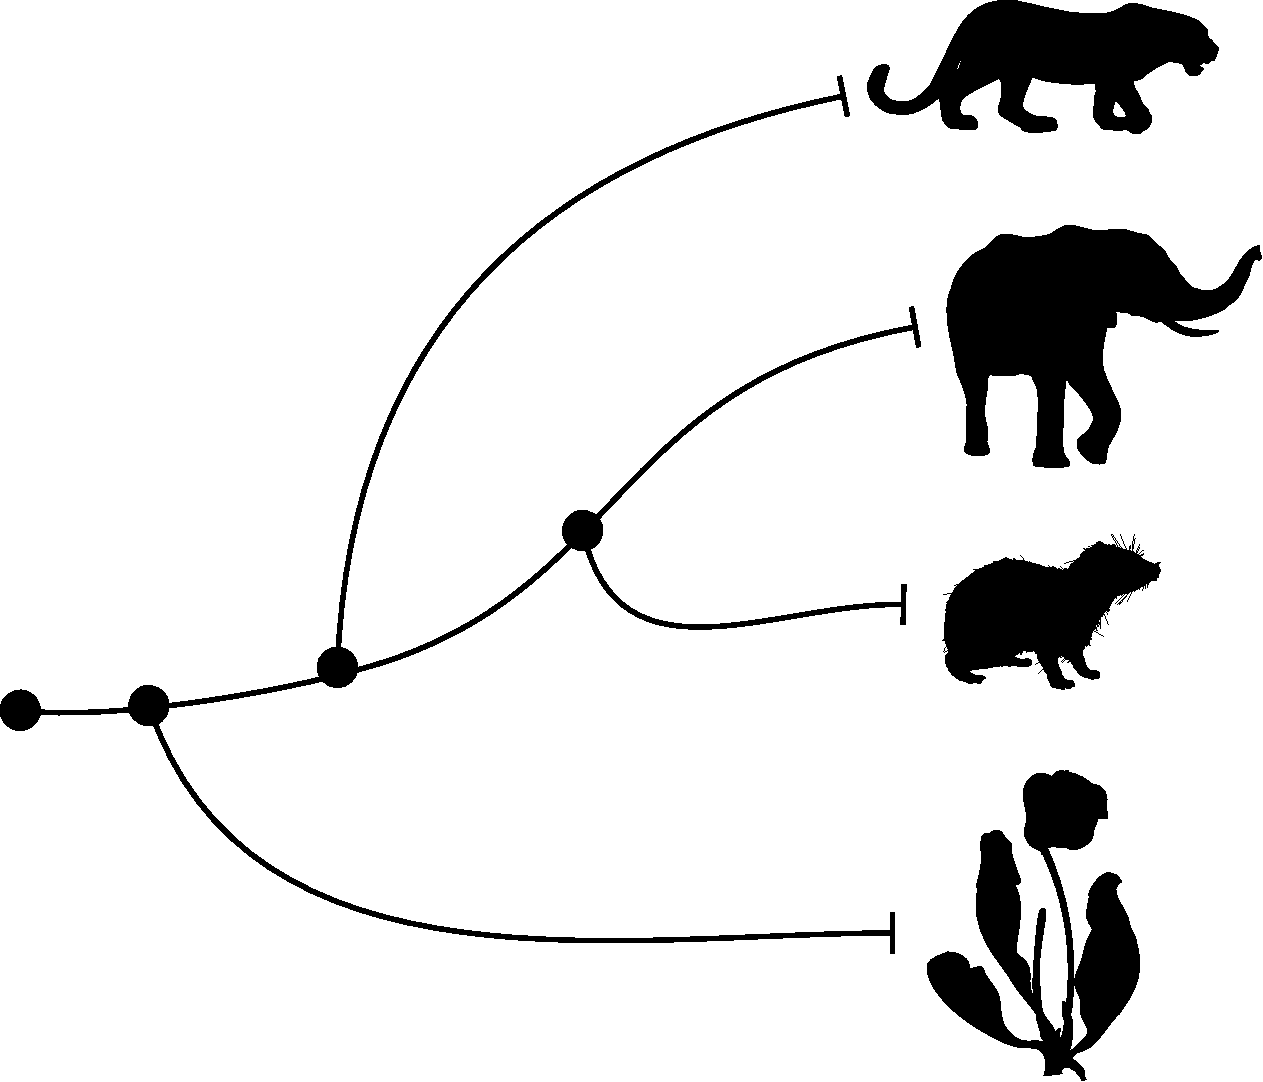
\includegraphics[width=0.4 \textwidth]{images/small_phylo.pdf} & 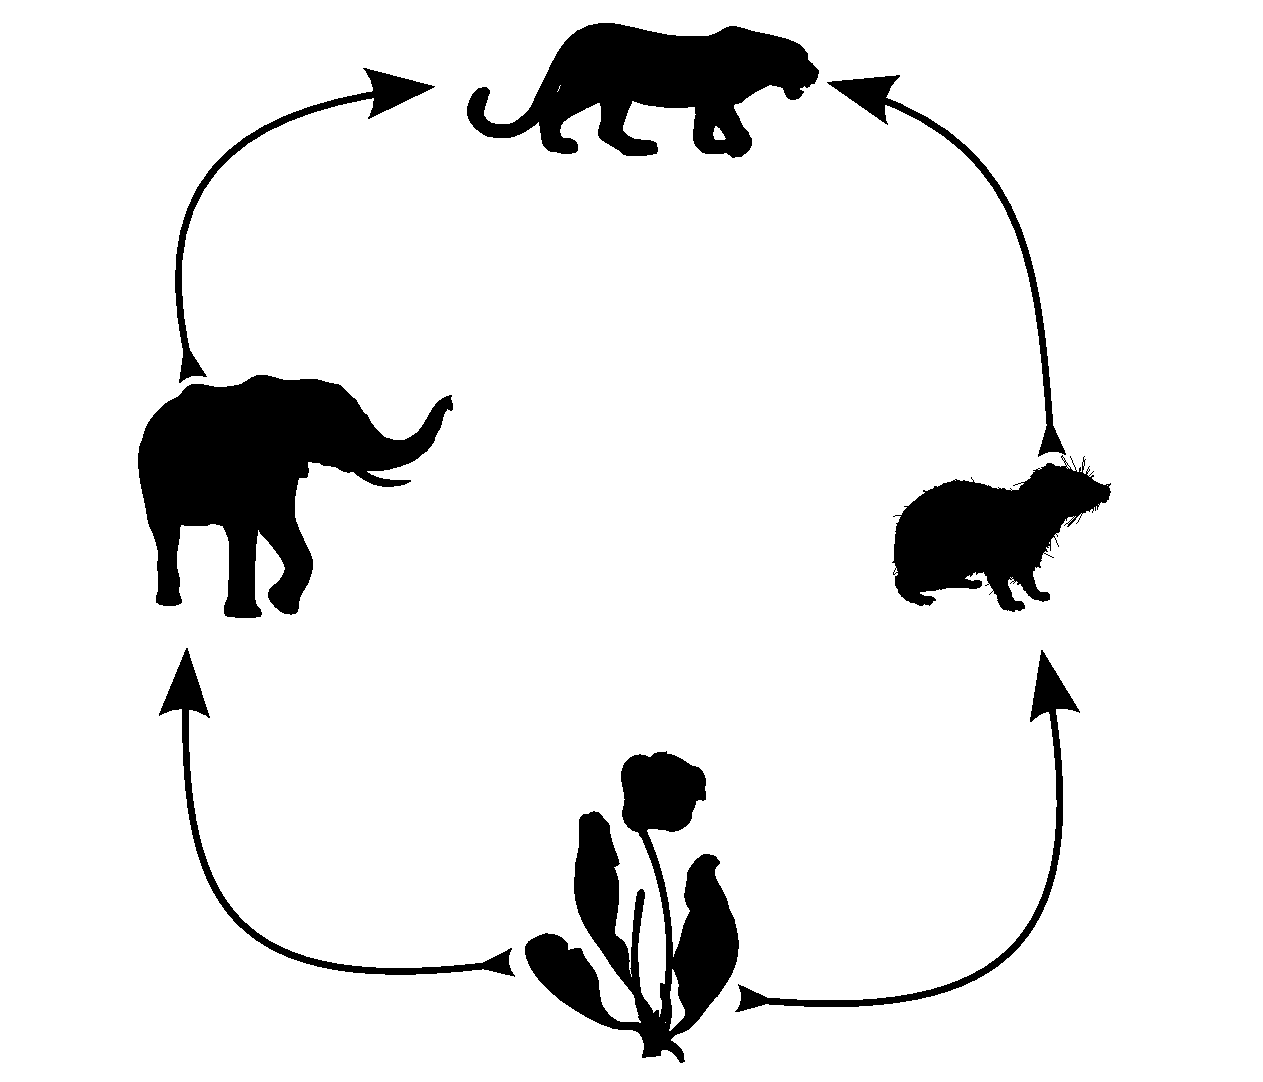
\includegraphics[width=0.4 \textwidth]{images/small_fw.pdf} \\ \hline
\end{tabular}

\end{frame}

\begin{frame}{Evolution in/of Ecology}

Evolution shaped the stochastic backbones of Food Webs

{[}Two images: Serengeti and Weddell{]}

\end{frame}

\begin{frame}{Food Webs embedded}

\begin{itemize}[<+->]
\centering
\item
Random Dot Product Graphs

  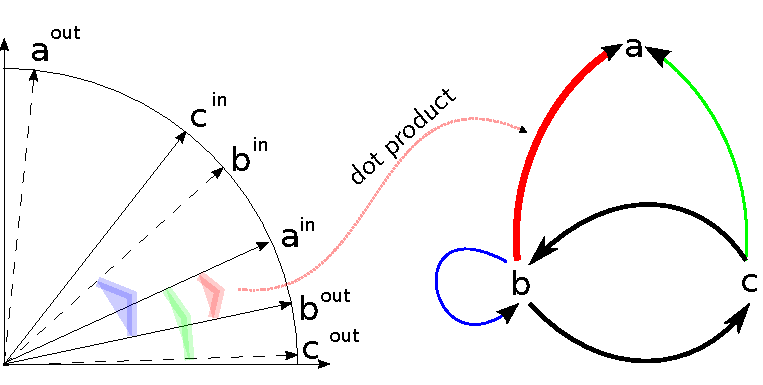
\includegraphics[width=0.4\linewidth]{images/RDPGmodel.pdf}

\item
Phylogenetic vs.~Observed traits
  \begin{equation*}
    \textrm{vcv}\left( \hat{x} | \tau, \mbox{model} \right) \mbox{ vs. } \textrm{vcv}\left(x\right)
  \end{equation*}

\end{itemize}

\end{frame}

\begin{frame}{More questions (than answers)}

\begin{itemize}[<+->]
\itemsep1pt\parskip0pt\parsep0pt
\item
  There is phylogenetic signal
\item
  It is quite weak
\item
  It saturates with dimensionality
\item
  Fine wirings may be deceiving
\item
  Evolutionary model is inadequate
\end{itemize}

\end{frame}

\begin{frame}{(Not a) Conclusion}

\begin{itemize}[<+->]
\item
  Spoiler 1: Evolutionary distinctiveness vs.~Web Centrality
\item
  Spoiler 2: An ecological informed model of species evolution maybe
  it's (almost) there.
\end{itemize}

\end{frame}

\begin{frame}{Thanks!}

\begin{centering}

Joint work with  
Daniel B. Stouffer (University of Canterbury)

Many thanks to  
Mike Steel; Carey Priebe; A. Mooers', D.B. Stouffer's \& J. Tylianakis's labs; ...

Funds by the Allan Wilson Centre for Molecular Ecology and Evolution.

\vspace{2cm}

\small{By the way, I'm looking for a postdoc.}

\end{centering}

\end{frame}

\end{document}
